\documentclass[a4paper, oneside]{article}
\usepackage[utf8]{inputenc}
\usepackage[ngerman]{babel}
\usepackage[top=2.5cm, bottom=3cm, outer=2.5cm, inner=2.5cm, heightrounded]{geometry}
\usepackage{graphicx}
\usepackage{morefloats}
\usepackage{wrapfig}
\usepackage{hyperref}
\usepackage{cite}
\usepackage{siunitx}
\usepackage[default]{sourcesanspro}
\usepackage[T1]{fontenc}
\usepackage{url}
\usepackage{marginnote}
\usepackage[font=footnotesize]{caption}
\usepackage{color}
\usepackage{xcolor}
\usepackage{multicol}
\usepackage[fleqn]{mathtools}
\usepackage{amssymb}
\usepackage{wrapfig}
\usepackage[noindentafter]{titlesec}
\usepackage{fancyhdr}
\usepackage{lastpage}
\usepackage{comment}

%% LÖSUNGEN ANZEIGEN
\newif\ifshow
%\showtrue
\showfalse

%%%SECTIONING
\renewcommand*{\marginfont}{\noindent\rule{0pt}{0.7\baselineskip}\footnotesize}

\newcommand{\aufgabe}[1]{\subsection{#1}}
\newcommand{\loesung}[1]{\subsubsection{#1}}

\newcommand{\simpleset}[1]{\ensuremath \left\{ #1 \right\}}
\newcommand{\ematrix}[2]{\renewcommand{\arraystretch}{1}\ensuremath\left(\begin{array}{@{}#1@{}}#2\end{array}\right)}

\renewcommand{\theenumi}{\alph{enumi})}
\renewcommand{\labelenumi}{\text{\theenumi}}

\newcounter{aufgabe}
%\newenvironment{lsg}{\loesung}{}
\ifshow
  \newenvironment{lsg}{\loesung}{}
\else
  \excludecomment{lsg}
\fi

\newenvironment{inhalt}
  {\paragraph{Inhalt des Übungsblatts:}\itemize\let\origitem\item}
  {\enditemize\vspace{2em}}

\newcommand{\R}{\ensuremath\mathbb{R}}
\newcommand{\N}{\ensuremath\mathbb{N}}
\newcommand{\Z}{\ensuremath\mathbb{Z}}
\newcommand{\LM}{\ensuremath\mathbb{L}}
\newcommand{\intd}{\ensuremath\mathrm{d}}
\newcommand{\e}{\ensuremath\mathrm{e}}
\renewcommand{\d}{\,\mathrm{d}}
\newcommand{\stf}[1]{\ensuremath \left[ #1 \right]}

\newcommand{\cas}{\hfill (CAS)}
\newcommand{\seite}[1]{\textit{(S. #1)}}

\newcommand{\vektor}[1]{\ensuremath\begin{pmatrix} #1 \end{pmatrix}}


\everymath{\displaystyle}

%Malpunkte
\mathcode`\*="8000
{\catcode`\*\active\gdef*{\cdot}}

%SECTION
\titleformat{\section}
{\clearpage\setcounter{aufgabe}{0}\vspace{1em}\Large\raggedright\bfseries}
{}
{0pt}
{}

\titleformat{\subsection}[runin]
{\stepcounter{aufgabe}\vspace{1px}\normalfont\raggedright\bfseries}
{A\theaufgabe: }
{0pt}
{\ }

\titleformat{\subsubsection}[runin]
{\normalfont\raggedright\bfseries}
{Lösung \theaufgabe: }
{0pt}
{\ }


%FANCYHDR
\pagestyle{fancy}
\lhead{\small Simon König\\ Joshua Fabian}
\rhead{\small Mathecrashkurs 2018}
\cfoot{Seite \thepage\thinspace von\thinspace\pageref{LastPage}}
\lfoot{}
\renewcommand{\headrulewidth}{0.5pt}
\renewcommand{\footrulewidth}{0pt}

\title{Mathe-Crashkurs 2018 - Übungsblatt}
\date{\today}
\author{Simon König, Joshua Fabian}

\chead{\Large Joshua Aufgabensammlung}


\begin{document}

<<<<<<< HEAD
\aufgabe{Lineare Gleichungssysteme}
Löse das Gleichungssystem:
\begin{alignat*}{4}
	-5x_1& +x_2& -x_3& = 7\\
	5x_1&  -3x_2& -2_3& = -11\\
	x_1& & x_3& =-1
\end{alignat*}
Interpretiere das LGS und die Lösungsmenge geometrisch.
=======

\aufgabe{Trigonometrie: }
\begin{enumerate}

\end{enumerate}
\begin{lsg}{}
	\begin{enumerate}

\end{lsg}




\aufgabe{Funktionenscharen: }
\begin{enumerate}
  \item Berechne die Nullstellen der Funktionenscharen in Abhängigkeit von $a\in \R, a\neq 0$:
  \begin{itemize}
    \item $f_a(x)=x^2+2ax+9$
    \item $g_a(x)=5ax+15a$
    \item $h_a(x)=x^3-a^2$
    \item $j_a(x)=(x-3a)(x+6a)$
  \end{itemize}
  \item Gegeben ist die Funktionenschar $f_a$ mit $f_a(x)=(x+a)*\e^{-x}\ , x\in \R$ .
  \begin{itemize}
    \item Untersuche die Lage des Maxmimums.
    \item Gib die Gleichung der Funktion an, auf der die Maxima aller Scharkurven liegen.
  \end{itemize}
\end{enumerate}
\begin{lsg}{}
	\begin{enumerate}
		\item \begin{itemize}
			\item $0=x^2+2ax+9 \rightsquigarrow x_1=\sqrt{a^2-9}-a,\ x_2=-\sqrt{a^2-9}-a$\\
			\item $0=5ax+15a \rightsquigarrow x=-3$\\
			\item $0=x^3-a^2 \rightsquigarrow x=\sqrt[3]{a^2}$\\
			\item $\text{Nullprodukt:}\ x_1=3a,\ x_2=-6a$
		\end{itemize}
		\item \begin{itemize}
			\item Ableitung bilden: \begin{align*}
				f'_a(x)&=\e^{-x}-x\e^{-x}-a\e^{-x}=(1-x-a)*\e^{-x}\\
				f''_a(x)&=-\e^{-x}-\e^{-x}+x\e^{-x}+a\e^{-x}=(a+x-2)*\e^{-x}
			\end{align*}\\
			Extremstelle: $f'_a(x)=0 \rightsquigarrow x=1-a$ \\
			In $f''_a$ einsetzen: $f''_a(1-a)=(a+1-a-2)*\e^{-(1-a)}<0$ für alle $a\in \R\Rightarrow $HP bei $x=1-a$\\
			HP bei $(1-a|\e^{a-1})$
			\item Aus dem HP bei $(1-a|\e^{a-1})$ folgt $x_{h}=1-a \rightsquigarrow a=1-x_{h}$\\
			Eingesetzt in $y_{h}=\e^{a-1}$ folgt: $y_h=\e^{-x_h}$ \\
			Damit gilt für die Ortskurve: $t(x)=\e^{-x}$

		\end{itemize}

	\end{enumerate}
\end{lsg}


\aufgabe{Integral: }
\begin{enumerate}
	\item Welche der Auswahlmöglichkeiten können eingesetzt werden?
	\begin{equation*}
		\int\limits_0^5 \left(3x^2+ \frac 1 5 x\right)  \d x = \Box
	\end{equation*}
  \begin{multicols}{4}
    \begin{itemize}
      \item $\stf{6x + \frac{1}{5}}_0^5$
      \item $\bigg[x^3 + 0,1 x^2\bigg]_0^5$
  		\item $127,5$
      \item $\stf{x^3 + \frac{1}{10} x^2}_1^6$
  	\end{itemize}
  \end{multicols}


	\item Bestimme $\int\limits_0^{\sqrt{\ln(2)}} 2x*\e^{(x^2)} \d x$
  \item Berechne den Gesamtinhalt der Flächen, die durch die Schaubilder der Funktionen $f$ und $g$ eingeschlossen wird:
  \begin{itemize}
    \item $f(x)=x^2, g(x)=2-x^2$
    \item $f(x)=x^3, g(x)=x^2$
    \item $f(x)=x^3, g(x)=x\ $ (Achtet auf Flächen über und unter der x-Achse)
  \end{itemize}
\end{enumerate}
\begin{lsg}{}
  \begin{enumerate}
    \item $\bigg[x^3 + 0,1 x^2\bigg]_0^5$ und $127,5$
    \item Kettenregel beim Ableiten: $(\e^{a(x)})'=a'(x)*\e^{a(x)}$, woraus hier folgt:\\ $\int\limits_0^{\sqrt{\ln(2)}} 2x*\e^{(x^2)} \d x = \left[\e^{(x^2)}\right]_0^{\sqrt{\ln(2)}}=2-1=1$
    \item
    \begin{itemize}
      \item Schnittpunkte der Graphen: $x_{1,2}=\pm 1$\\ $\int\limits_{-1}^1 2-x^2-x^2\d x=\left[2x-\frac{2}{3}x^3\right]_{-1}^1=\frac 8 3$
      \item Schnittpunkt der Graphen: $x_1=0,\ x_2=1$ \\$\int_0^1 (x^2-x^3)\d x=\left[\frac{1}{3}x^3-\frac{1}{4}x^4\right]_0^1=\frac 1 {12}$
      \item Schnittpunkte der Graphen: $x_{1,2}=\pm 1,\ x_3=0$ \\$\int_{-1}^0 (x^3-x)\d x+\int_0^1 (x-x^3)\d x=2*\left[\frac{1}{2}x^2-\frac{1}{4}x^4\right]_0^1=\frac 1 2$
    \end{itemize}
  \end{enumerate}
\end{lsg}





>>>>>>> origin/master



\aufgabe{Winkelberechnung}
\begin{enumerate}
	\item Berechnen Sie die Schnittwinkel der beiden Geraden $g_i$ und $h_i$:
	\begin{itemize}
		\item $g_1: \vec x = \vektor{2\\2\\-3} + r*\vektor{2\\1\\-1}$ und $h_1: \vec x = \vektor{3\\0\\-1} + s* \vektor{1\\-2\\2}$
		\item
	\end{itemize}
	\item
\end{enumerate}

\aufgabe{Lageberechnungen}
\begin{enumerate}
	\item enum
	\item	enum
\end{enumerate}

\aufgabe{Abstandsberechnung}
\begin{enumerate}
	\item enum
	\item	enum
\end{enumerate}


\aufgabe{Winkelberechnung}
\begin{enumerate}
	\item enum
	\item	enum
\end{enumerate}



\aufgabe{Graphanalyse: } (vgl. Abitur 2015)
\begin{multicols}{2}
	Die Abbildung zeigt den Graphen der Ableitungsfunktion $f'$ einer ganzrationalen Funktion $f$.
	Entscheide ob die folgenden Aussagen wahr oder falsch sind. Begründe jeweils Deine Antwort.
	\begin{enumerate}
		\item Der Graph von $f$ hat bei $x=-3$ einen Tiefpunkt.
		\item $f(-2)<f(-1)$
		\item $f''(-2)+f'(-2)<1$
		\item Der Grad der Funktion $f$ ist mindestens vier.
	\end{enumerate}
	\columnbreak

	\centering
	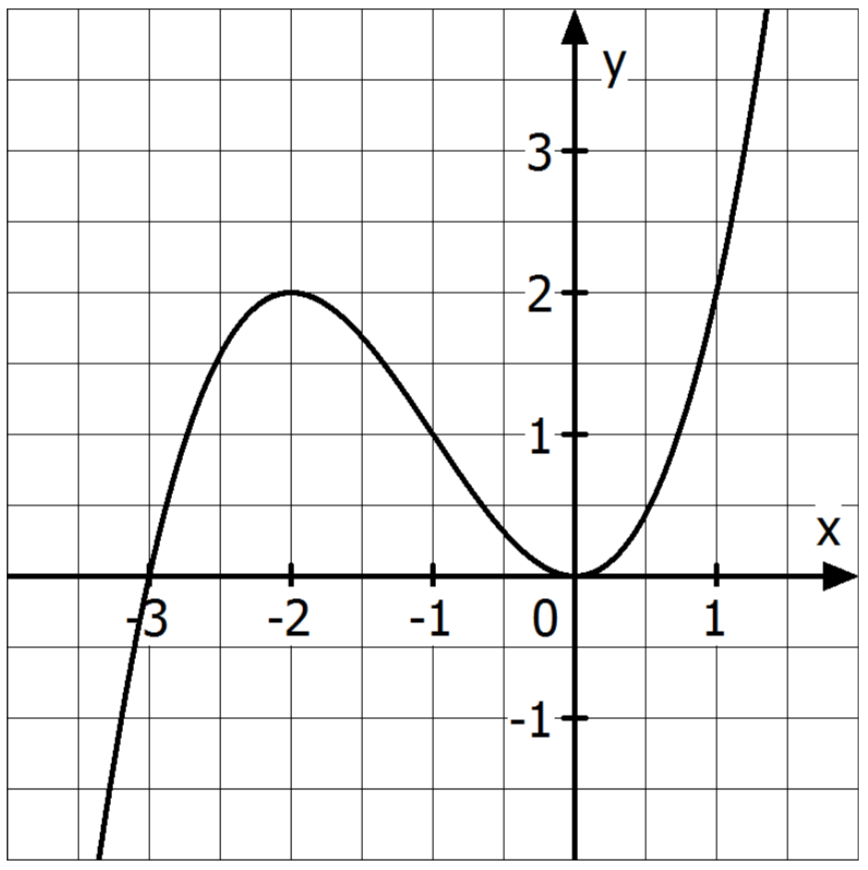
\includegraphics[width=0.7\linewidth]{Graphanalyse.png}
\end{multicols}

\begin{lsg}{}
	\begin{enumerate}
		\item Wahr, Vorzeichenwechsel bei $x=-3$
		\item Wahr, streng monoton steigend im Intervall $[-2;-1]$
		\item Falsch, $f''(-2)+f'(-2)=0+2>1$
		\item Wahr, $f'$ besitzt zwei Extrempunkte $\rightsquigarrow f''$ ist mindestens vom Grad 2. Der Graph der Abbildung könnte auch drei Nullstellen haben, $f'$ ist also mindestens vom Grad 3.
	\end{enumerate}
\end{lsg}



\aufgabe{Extrempunkte}

\begin{lsg}{}
	
\end{lsg}


\end{document}
